\subsection{Solving pocket Rubik’s cube (2*2*2) using Z3}
\label{PocketCubeSMT}

\begin{figure}[H]
\centering
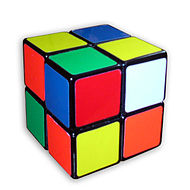
\includegraphics[scale=0.75]{SMT/rubik2/failed/190px-Pocket_cube_scrambled.jpg}
\caption{Pocket cube}
\end{figure}

( The image has been taken \href{https://en.wikipedia.org/wiki/Pocket_Cube}{from Wikipedia}. )

Solving Rubik's cube is not a problem, finding shortest solution is.

\subsubsection{Intro}

First, a bit of terminology.
There are 6 colors we have: white, green, blue, orange, red, yellow.
We also have 6 sides: front, up, down, left, right, back.

This is how we will name all facelets:

% TODO TikZ
\begin{lstlisting}
        U1 U2
        U3 U4

       -------
L1 L2 | F1 F2 | R1 R2 | B1 B2
L3 L4 | F3 F4 | R3 R4 | B3 B4
       -------

        D1 D2
        D3 D4
\end{lstlisting}

Colors on a solved cube are:

\begin{lstlisting}
    G G
    G G
    ---
R R|W W|O O|Y Y
R R|W W|O O|Y Y
    ---
    B B
    B B
\end{lstlisting}

There are 6 possible turns: front, left, right, back, up, down.
But each turn can be clockwise, counterclockwise and half-turn (equal to two CW or two CCW).
Each CW is equal to 3 CCW and vice versa.
Hence, there are 6*3=18 possible turns.

It is known, that 11 turns (including half-turns) are enough to solve any pocket cube
(\href{https://en.wikipedia.org/wiki/Optimal_solutions_for_Rubik%27s_Cube}{God’s algorithm}).
This means, \href{http://mathworld.wolfram.com/GraphDiameter.html}{graph has a diameter} of 11.
For 3*3*3 cube one need 20 turns (\url{http://www.cube20.org/}).
See also: \url{https://en.wikipedia.org/wiki/Rubik%27s_Cube_group}.

\subsubsection{Z3}

There are 6 sides and 4 facelets on each, hence, 6*4=24 variables we need to define a state.

Then we define how state is transformed after each possible turn:

\begin{lstlisting}
FACE_F, FACE_U, FACE_D, FACE_R, FACE_L, FACE_B = 0,1,2,3,4,5

def rotate_FCW(s):
    return [
        [ s[FACE_F][2], s[FACE_F][0], s[FACE_F][3], s[FACE_F][1] ],   # for F
        [ s[FACE_U][0], s[FACE_U][1], s[FACE_L][3], s[FACE_L][1] ],   # for U
        [ s[FACE_R][2], s[FACE_R][0], s[FACE_D][2], s[FACE_D][3] ],   # for D
        [ s[FACE_U][2], s[FACE_R][1], s[FACE_U][3], s[FACE_R][3] ],   # for R
        [ s[FACE_L][0], s[FACE_D][0], s[FACE_L][2], s[FACE_D][1] ],   # for L
        [ s[FACE_B][0], s[FACE_B][1], s[FACE_B][2], s[FACE_B][3] ] ]  # for B

def rotate_FH(s):
    return [
        [ s[FACE_F][3], s[FACE_F][2], s[FACE_F][1], s[FACE_F][0] ],
        [ s[FACE_U][0], s[FACE_U][1], s[FACE_D][1], s[FACE_D][0] ],
        [ s[FACE_U][3], s[FACE_U][2], s[FACE_D][2], s[FACE_D][3] ],
        [ s[FACE_L][3], s[FACE_R][1], s[FACE_L][1], s[FACE_R][3] ],
        [ s[FACE_L][0], s[FACE_R][2], s[FACE_L][2], s[FACE_R][0] ],
        [ s[FACE_B][0], s[FACE_B][1], s[FACE_B][2], s[FACE_B][3] ] ]

...
\end{lstlisting}

Then we define a function, which takes turn number and transforms a state:

\begin{lstlisting}
# op is turn number
def rotate(turn, state, face, facelet):
    return If(op==0,  rotate_FCW (state)[face][facelet],
           If(op==1,  rotate_FCCW(state)[face][facelet],
           If(op==2,  rotate_UCW (state)[face][facelet],
           If(op==3,  rotate_UCCW(state)[face][facelet],
           If(op==4,  rotate_DCW (state)[face][facelet],

...

           If(op==17, rotate_BH  (state)[face][facelet],
                      0))))))))))))))))))
\end{lstlisting}

Now set "solved" state, initial state and connect everything:

\begin{lstlisting}
move_names=["FCW", "FCCW", "UCW", "UCCW", "DCW", "DCCW", "RCW", "RCCW", "LCW", "LCCW", "BCW", "BCCW", "FH", "UH", "DH", "RH", "LH", "BH"]

def colors_to_array_of_ints(s):
    return [{"W":0, "G":1, "B":2, "O":3, "R":4, "Y":5}[c] for c in s]

def set_current_state (d):
    F=colors_to_array_of_ints(d["FACE_F"])
    U=colors_to_array_of_ints(d["FACE_U"])
    D=colors_to_array_of_ints(d["FACE_D"])
    R=colors_to_array_of_ints(d["FACE_R"])
    L=colors_to_array_of_ints(d["FACE_L"])
    B=colors_to_array_of_ints(d["FACE_B"])
    return F,U,D,R,L,B # return tuple

# 4
init_F, init_U, init_D, init_R, init_L, init_B=set_current_state({"FACE_F":"RYOG", "FACE_U":"YRGO", "FACE_D":"WRBO", "FACE_R":"GYWB", "FACE_L":"BYWG", "FACE_B":"BOWR"})

...

for TURNS in range(1,12): # 1..11
    print "turns=", TURNS

    s=Solver()

    state=[[[Int('state%d_%d_%d' % (n, side, i)) for i in range(FACELETS)] for side in range(FACES)] for n in range(TURNS+1)]
    op=[Int('op%d' % n) for n in range(TURNS+1)]

    for i in range(FACELETS):
        s.add(state[0][FACE_F][i]==init_F[i])
        s.add(state[0][FACE_U][i]==init_U[i])
        s.add(state[0][FACE_D][i]==init_D[i])
        s.add(state[0][FACE_R][i]==init_R[i])
        s.add(state[0][FACE_L][i]==init_L[i])
        s.add(state[0][FACE_B][i]==init_B[i])

    # solved state
    for face in range(FACES):
        for facelet in range(FACELETS):
            s.add(state[TURNS][face][facelet]==face)

    # turns:
    for turn in range(TURNS):
        for face in range(FACES):
            for facelet in range(FACELETS):
                s.add(state[turn+1][face][facelet]==rotate(op[turn], state[turn], face, facelet))

    if s.check()==sat:
        print "sat"
        m=s.model()
        for turn in range(TURNS):
            print move_names[int(str(m[op[turn]]))]
        exit(0)
\end{lstlisting}

% FIXME URL
( The full source code: \url{https://github.com/dennis714/yurichev.com/blob/master/blog/rubik/rubik2_z3.py} )

That works:

\begin{lstlisting}
turns= 1
turns= 2
turns= 3
turns= 4
sat
RCW
UCW
DCW
RCW
\end{lstlisting}

...but very slow. It takes up to 1 hours to find a path of 8 turns, which is not enough, we need 11.

Nevetheless, I decided to include Z3 solver as a demonstration.

See also: solving pocket cube using SAT solver: \ref{PocketCubeSAT}.

